% Phase I report - IEEE conference format
% Build:  pdflatex report_phase1.tex   (run twice; needs datapath.pdf in this folder)
\documentclass[conference]{IEEEtran}
\usepackage{graphicx}
\usepackage{booktabs}
\usepackage{array}
\usepackage{cite}
\usepackage{url}

\begin{document}

\title{Design and Verification of a Single-Cycle RV32I Processor in Verilog\\
{\large Phase I Report --- CSA-222 Modern Computer Architecture}}

\author{\IEEEauthorblockN{Rishi Raj (2401010380), Yash Yadav (2401010514), Aditya Samadhiya (2401010037),\\
Kaustubh Mishra (2401020116) and Yash Raj (2401010514)}
\IEEEauthorblockA{B.Tech Computer Science and AI, Batch 2024\\
Newton School of Technology, Rishihood University\\
Sonipat, Haryana, India}}

\maketitle

\begin{abstract}
This report describes Phase I of a project to build a compact single-cycle
processor that executes a ten-instruction subset of the RISC-V RV32I base
instruction set: ADD, SUB, AND, OR, XOR, ADDI, LW, SW, BEQ and BNE. The
processor is written in synthesizable Verilog as eleven small modules that
mirror the textbook datapath: a program counter, instruction memory, control
unit, register file, immediate generator, ALU with its own decoder, data
memory and the adders and multiplexers that connect them. Every module has a
self-checking testbench, and the integrated processor has been simulated in
Icarus Verilog running two hand-assembled test programs. Both programs finish
with the register and memory contents that were worked out by hand
beforehand. Phase II will widen the test coverage, synthesize the design and
report resource usage and timing.
\end{abstract}

\begin{IEEEkeywords}
RISC-V, RV32I, single-cycle processor, datapath, control unit, Verilog
\end{IEEEkeywords}

% ---------------------------------------------------------------------------
\section{Introduction}
Every program eventually runs as a sequence of fetch, decode and execute steps
on a processor. The simplest hardware that can do this is the single-cycle
processor, in which each instruction completes within one clock period. It is
not how fast commercial processors are built, but every later idea in the
course, including pipelining, hazards and forwarding, is a modification of
this design, so building it is the most direct way to understand the others.

We chose RISC-V as the instruction set because it is an open standard, its
base integer subset is small, and its instruction formats were designed to
make decoding simple. The course labs introduce datapaths through MIPS32;
RISC-V follows the same load-store philosophy, so the concepts carry over
directly while the encoding details are new.

The goal of the full project is a working processor with RTL, testbenches,
waveforms, test programs and a synthesis report. Phase I covers the design,
the RTL for every module and simulation of the integrated processor.

% ---------------------------------------------------------------------------
\section{Literature Review}

\subsection{RISC and the RISC-V instruction set}
Patterson and Ditzel argued in 1980 that a small set of simple, regular
instructions leads to simpler hardware and a shorter design time than a large
complex instruction set \cite{patterson1980}. RISC-V, started at UC Berkeley
in 2010, applies that idea as a free and open standard \cite{asanovic2014}.
The specification defines a small base integer ISA, RV32I, and keeps
everything else (multiplication, floating point, compressed instructions) in
optional extensions \cite{riscvspec}. RV32I has 32 registers of 32 bits with
\texttt{x0} fixed at zero, fixed 32-bit instructions, and a handful of
formats in which the register fields and the sign bit of the immediate always
sit in the same bit positions. These choices matter for this project: the
register file can be read before the instruction type is known, and sign
extension always uses bit~31.

\subsection{Textbook single-cycle designs}
Patterson and Hennessy develop a single-cycle datapath step by step for a
subset of load, store, arithmetic-logical and branch instructions, and
introduce the two-level control scheme in which a main decoder produces a
2-bit ALU operation class and a second small decoder turns it into the exact
ALU function \cite{patterson2020}. Harris and Harris present a similar
RISC-V single-cycle processor and give complete HDL for it
\cite{harris2021}. Both texts point out the main weakness of the approach:
the clock period has to fit the slowest instruction, the load, so every other
instruction wastes time. This is the motivation for multi-cycle and pipelined
designs, which are outside the scope of this project. Nisan and Schocken take
the same build-it-from-small-parts approach from logic gates up to a complete
computer \cite{nisan2021}, which influenced how we split the work into small
independently testable modules.

\subsection{Open-source RISC-V cores}
Several open cores show what the design space looks like beyond the textbook.
PicoRV32 is a size-optimized multi-cycle core that trades cycles per
instruction for a small area and a high clock frequency \cite{picorv32}. SERV
goes further and processes data one bit at a time to minimize area
\cite{serv}. Ibex is a production-quality two-stage pipelined core with
extensive verification \cite{ibex}. These cores optimize for area,
frequency or robustness and are correspondingly harder to read. Our design
optimizes for clarity instead: one module per block of the datapath diagram,
no pipelining, and only the instructions needed to demonstrate arithmetic,
memory access and control flow.

\subsection{Tools}
The design is simulated with Icarus Verilog \cite{iverilog} and waveforms are
viewed in GTKWave \cite{gtkwave}, the same tool flow used in the course labs.

% ---------------------------------------------------------------------------
\section{Proposed Solution}

\subsection{Instruction subset}
Table~\ref{tab:instr} lists the ten supported instructions. They cover four
of the RV32I formats. R-type instructions operate on two registers. I-type
instructions (ADDI and LW) take one register and a 12-bit immediate. The
S-type store splits its immediate across two fields so that the register
fields stay in place. The B-type branches encode a 13-bit offset whose lowest
bit is always zero.

\begin{table}[!htb]
\caption{Supported instructions and their encodings}
\label{tab:instr}
\centering
\begin{tabular}{llccc}
\toprule
Instr. & Format & opcode & funct3 & funct7 \\
\midrule
ADD  & R & 0110011 & 000 & 0000000 \\
SUB  & R & 0110011 & 000 & 0100000 \\
AND  & R & 0110011 & 111 & 0000000 \\
OR   & R & 0110011 & 110 & 0000000 \\
XOR  & R & 0110011 & 100 & 0000000 \\
ADDI & I & 0010011 & 000 & --- \\
LW   & I & 0000011 & 010 & --- \\
SW   & S & 0100011 & 010 & --- \\
BEQ  & B & 1100011 & 000 & --- \\
BNE  & B & 1100011 & 001 & --- \\
\bottomrule
\end{tabular}
\end{table}

\begin{figure*}[t]
\centering
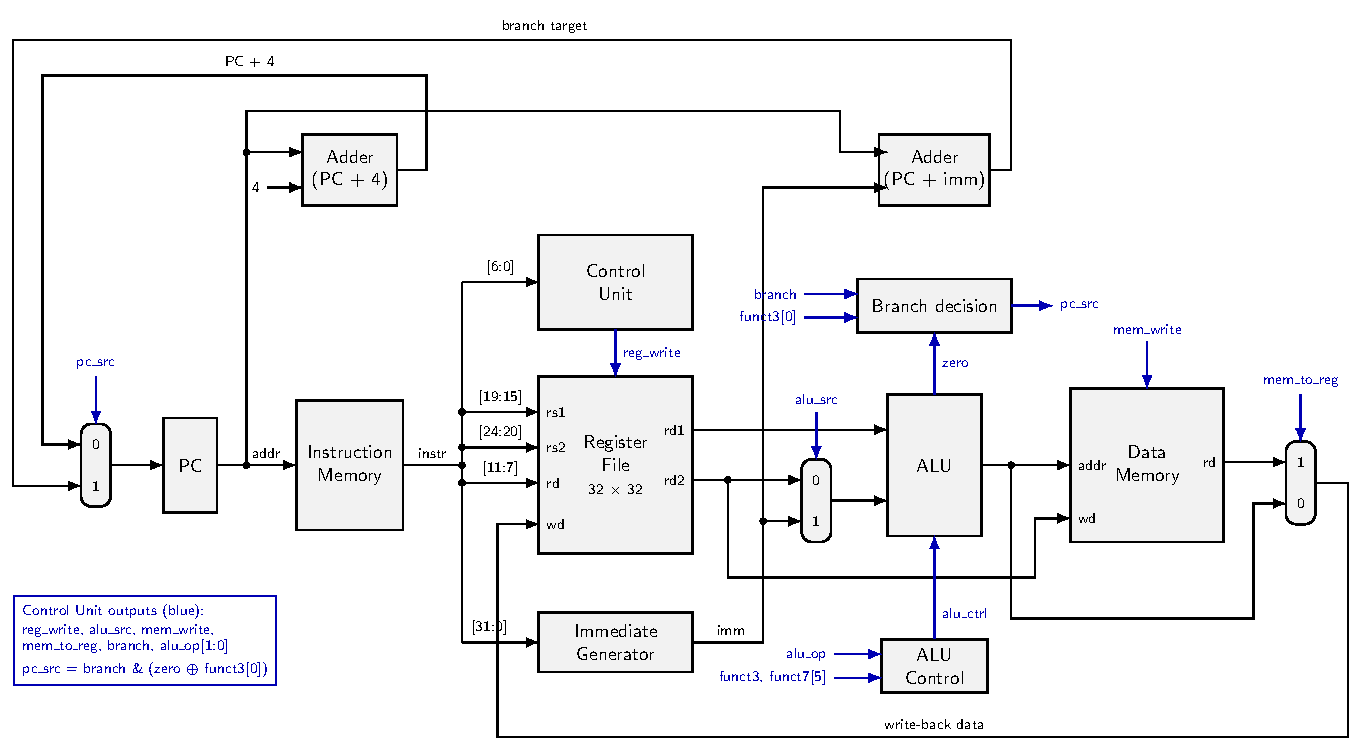
\includegraphics[width=0.95\textwidth]{datapath.pdf}
\caption{Datapath of the single-cycle RV32I processor. Data signals are drawn
in black and control signals in blue.}
\label{fig:datapath}
\end{figure*}

\subsection{Datapath}
Fig.~\ref{fig:datapath} shows the datapath. One instruction moves through it
from left to right in a single clock cycle.

\textit{Fetch.} The program counter (PC) holds the address of the current
instruction. The instruction memory is read combinationally, and an adder
computes PC\,+\,4.

\textit{Decode.} The opcode goes to the control unit. The \texttt{rs1} and
\texttt{rs2} fields address the register file, which returns both values
combinationally. The immediate generator extracts and sign-extends the
immediate according to the instruction format.

\textit{Execute.} A multiplexer selects either the second register value or
the immediate as the second ALU operand. The ALU adds, subtracts or performs
AND, OR or XOR, and raises a \texttt{zero} flag when the result is zero. A
second adder computes the branch target PC\,+\,immediate.

\textit{Memory.} For LW and SW the ALU result is the memory address. Data
memory is read combinationally and written on the clock edge.

\textit{Write-back.} A multiplexer selects the ALU result or the memory data
and sends it back to the register file, which is written on the clock edge.

Only three things change on the clock edge: the PC, one register and one
memory word. Everything else is combinational logic, which is what makes the
design single-cycle.

\subsection{Control}
Control is split into two levels, following \cite{patterson2020}. The main
control unit looks only at the opcode and produces the signals in
Table~\ref{tab:control}. The ALU control block then uses the 2-bit
\texttt{alu\_op} together with \texttt{funct3} and bit 5 of \texttt{funct7}
to pick the ALU operation. ADD and SUB differ only in that \texttt{funct7}
bit; for ADDI the same bit position belongs to the immediate, so subtraction
is selected only when the opcode is R-type.

Branches reuse the ALU: it subtracts the two registers, and
\texttt{zero}\,=\,1 means they are equal. BEQ and BNE differ only in
\texttt{funct3[0]}, so the next-PC select is
\[
\texttt{pc\_src} = \texttt{branch} \cdot (\texttt{zero} \oplus \texttt{funct3[0]}).
\]
An unknown opcode leaves every write enable at zero, so it cannot corrupt
registers or memory.

\begin{table}[!htb]
\caption{Main control unit truth table (x = don't care)}
\label{tab:control}
\centering
\setlength{\tabcolsep}{3.5pt}
\begin{tabular}{lcccccc}
\toprule
Class & \rotatebox{70}{reg\_write} & \rotatebox{70}{alu\_src} &
\rotatebox{70}{mem\_write} & \rotatebox{70}{mem\_to\_reg} &
\rotatebox{70}{branch} & \rotatebox{70}{alu\_op} \\
\midrule
R-type    & 1 & 0 & 0 & 0 & 0 & 10 \\
ADDI      & 1 & 1 & 0 & 0 & 0 & 10 \\
LW        & 1 & 1 & 0 & 1 & 0 & 00 \\
SW        & 0 & 1 & 1 & x & 0 & 00 \\
BEQ / BNE & 0 & 0 & 0 & x & 1 & 01 \\
\bottomrule
\end{tabular}
\end{table}

\subsection{RTL structure}
Each block in Fig.~\ref{fig:datapath} is one Verilog module: \texttt{pc},
\texttt{adder}, \texttt{instr\_mem}, \texttt{control\_unit},
\texttt{reg\_file}, \texttt{imm\_gen}, \texttt{alu\_control}, \texttt{alu},
\texttt{mux2}, \texttt{data\_mem}, and the top level \texttt{rv32i\_top}
which only wires them together. Both memories hold 64 words. The instruction
memory is initialized from a hex file with \texttt{\$readmemh}, so a new
program can be run without touching the RTL. Programs are written in RISC-V
assembly and assembled by hand into hex; each hex line carries the assembly
as a comment.

\subsection{Verification and current status}
Every module has a self-checking testbench that applies inputs, compares the
outputs against expected values and prints a pass or fail summary.
Table~\ref{tab:tests} summarizes them. All checks pass in Icarus Verilog.

\begin{table}[!htb]
\caption{Testbenches and Phase I simulation status}
\label{tab:tests}
\centering
\begin{tabular}{@{}l>{\raggedright\arraybackslash}p{4.3cm}c@{}}
\toprule
Testbench & What is checked & Checks \\
\midrule
\texttt{tb\_fetch}   & reset, PC\,+\,4 stepping, jump to target, instruction read & 7 \\
\texttt{tb\_reg\_file} & write and read, dual read ports, write enable, \texttt{x0} stays zero & 35 \\
\texttt{tb\_imm\_gen} & I, S and B immediates, positive and negative & 11 \\
\texttt{tb\_alu}     & five ALU operations, zero flag, ALU decoder for all ten instructions & 21 \\
\texttt{tb\_control\_unit} & control table, unknown opcodes, multiplexer & 9 \\
\texttt{tb\_data\_mem} & write and read back, write enable, address range & 9 \\
\texttt{tb\_rv32i\_top} & program 1 and program 2 final state & 23 \\
\bottomrule
\end{tabular}
\end{table}

The integrated processor runs two programs. Program~1 uses ADDI, ADD, SUB,
AND, OR, XOR, SW and LW on the values 10 and 6, including a negative
immediate, and reaches its halt instruction after 14 cycles. Program~2 adds
the numbers 5 down to 1 in a loop and reaches halt after 24 cycles; it
exercises BNE and BEQ in both the taken and not-taken directions and ends
with a self-check that sets \texttt{x6} to 1 only if the sum read back from
memory equals 15. Table~\ref{tab:results} compares the simulated final state
with the values computed by hand. They match in every case.

\begin{table}[!htb]
\caption{Expected and simulated final state}
\label{tab:results}
\centering
\begin{tabular}{llcc}
\toprule
Program & Location & Expected & Simulated \\
\midrule
1 & \texttt{x3} (10 + 6)     & 16 & 16 \\
1 & \texttt{x4} (10 $-$ 6)   & 4  & 4 \\
1 & \texttt{x5} (10 AND 6)   & 2  & 2 \\
1 & \texttt{x6} (10 OR 6)    & 14 & 14 \\
1 & \texttt{x7} (10 XOR 6)   & 12 & 12 \\
1 & \texttt{x8} (ADDI $-$3)  & $-$3 & $-$3 \\
1 & \texttt{x11} (sum of loads) & 20 & 20 \\
1 & \texttt{mem[8]}          & 20 & 20 \\
2 & \texttt{x2} (loop sum)   & 15 & 15 \\
2 & \texttt{x6} (self-check) & 1  & 1 \\
2 & \texttt{mem[0]}          & 15 & 15 \\
\bottomrule
\end{tabular}
\end{table}

\subsection{Plan for Phase II}
The remaining work is: (1) more test programs aimed at corner cases such as
maximum and minimum immediates, forward and backward branches at the edges of
the offset range, and writes to \texttt{x0}; (2) synthesis of the design and a
resource report; (3) an estimate of the critical path and maximum clock
frequency, with a discussion of why the load instruction sets it;
(4) deployment on an FPGA board if one is available; and (5) the results and
discussion sections of the final report.

% ---------------------------------------------------------------------------
\section{Individual Contributions}
The work was divided so that each member owns a part of the datapath together
with its testbench, one section of this report and one segment of the demo
video. Table~\ref{tab:contrib} lists the split.

\begin{table}[!htb]
\caption{Individual contributions in Phase I}
\label{tab:contrib}
\centering
\setlength{\tabcolsep}{3pt}
\begin{tabular}{@{}p{2.3cm}>{\raggedright\arraybackslash}p{3.4cm}>{\raggedright\arraybackslash}p{2.3cm}@{}}
\toprule
Member & RTL and verification & Report and other \\
\midrule
Rishi Raj\newline(2401010380) & \texttt{pc}, \texttt{adder}, \texttt{instr\_mem}, \texttt{tb\_fetch};
           both test programs, hand-assembled & Abstract, Introduction \\
\addlinespace
Yash Yadav\newline(2401010514) & \texttt{reg\_file}, \texttt{imm\_gen} and their two testbenches &
           Literature Review \\
\addlinespace
Aditya Samadhiya\newline(2401010037) & \texttt{alu}, \texttt{alu\_control}, \texttt{tb\_alu} &
           Instruction subset, Datapath, block diagram \\
\addlinespace
Kaustubh Mishra\newline(2401020116) & \texttt{control\_unit}, \texttt{mux2}, \texttt{tb\_control\_unit} &
           Control section and truth table \\
\addlinespace
Yash Raj\newline(2401010514) & \texttt{data\_mem}, \texttt{rv32i\_top} integration,
           \texttt{tb\_data\_mem}, \texttt{tb\_rv32i\_top} &
           Verification section, repository, video editing \\
\bottomrule
\end{tabular}
\end{table}

% ---------------------------------------------------------------------------
\begin{thebibliography}{00}
\bibitem{patterson1980} D. A. Patterson and D. R. Ditzel, ``The case for the
reduced instruction set computer,'' \emph{ACM SIGARCH Comput. Archit. News},
vol. 8, no. 6, pp. 25--33, Oct. 1980.
\bibitem{asanovic2014} K. Asanovi\'c and D. A. Patterson, ``Instruction sets
should be free: The case for RISC-V,'' EECS Dept., Univ. California, Berkeley,
Tech. Rep. UCB/EECS-2014-146, Aug. 2014.
\bibitem{riscvspec} A. Waterman and K. Asanovi\'c, Eds., \emph{The RISC-V
Instruction Set Manual, Volume I: Unprivileged ISA}, Document Version
20191213, RISC-V Foundation, Dec. 2019.
\bibitem{patterson2020} D. A. Patterson and J. L. Hennessy, \emph{Computer
Organization and Design RISC-V Edition: The Hardware Software Interface},
2nd ed. Cambridge, MA, USA: Morgan Kaufmann, 2020.
\bibitem{harris2021} S. L. Harris and D. M. Harris, \emph{Digital Design and
Computer Architecture: RISC-V Edition}. Cambridge, MA, USA: Morgan Kaufmann,
2021.
\bibitem{nisan2021} N. Nisan and S. Schocken, \emph{The Elements of Computing
Systems: Building a Modern Computer from First Principles}, 2nd ed.
Cambridge, MA, USA: MIT Press, 2021.
\bibitem{picorv32} C. Wolf, ``PicoRV32: A size-optimized RISC-V CPU.''
[Online]. Available: \url{https://github.com/YosysHQ/picorv32}
\bibitem{serv} O. Kindgren, ``SERV: The serial RISC-V CPU.'' [Online].
Available: \url{https://github.com/olofk/serv}
\bibitem{ibex} lowRISC, ``Ibex RISC-V core.'' [Online]. Available:
\url{https://github.com/lowRISC/ibex}
\bibitem{iverilog} S. Williams, ``Icarus Verilog.'' [Online]. Available:
\url{https://steveicarus.github.io/iverilog/}
\bibitem{gtkwave} T. Bybell, ``GTKWave.'' [Online]. Available:
\url{https://gtkwave.sourceforge.net/}
\end{thebibliography}

\end{document}

